\label{sec:anchor}Đồ án đưa đặc trưng lịch sử của HiGBDT vào bài toán cập nhật của \Cref{sec:mo_rong}: ước lượng SOH ở các chu kỳ không đo từ lần đo dung lượng gần nhất, trên cùng fold với các thí nghiệm khác, 30\,\% nhãn, $L$ và chuẩn hoá tính trên cell huấn luyện. GBDT-cập nhật dùng đặc trưng sạc hiện tại và độ đổi của chúng kể từ lần đo, SOH ở lần đo, khoảng chu kỳ tới lần đo và độ dốc giữa hai lần đo gần nhất. Hai mô hình dùng lịch sử thêm hai trung bình trượt mũ nhân quả của đặc trưng sạc ($\rho = 0{,}1$ và $0{,}03$), log khoảng chu kỳ và chỉ số chu kỳ: HiGBDT-$\Delta$ học độ giảm SOH kể từ lần đo, HiGBDT-R học phần dư so với ngoại suy tuyến tính từ hai lần đo gần nhất. HiGBDT-V chọn trên tập xác thực, theo từng lịch đo, một trong ba mô hình đó và trọng số trộn nó với giữ lần đo hoặc ngoại suy tuyến tính. Mỗi mô hình học trên tối đa khoảng 60 nghìn cặp (chu kỳ, lần đo), cân theo cell và lịch đo, có thêm hai pha đo ngẫu nhiên cho mỗi lịch thưa. Số cây chọn trên tập xác thực. \Cref{tab:anchor} cho kết quả. Chỉ với một lần đo mỗi $0{,}2L$ chu kỳ, GBDT-cập nhật đạt MAE 1{,}27--6{,}12 ($\times10^{-3}$), bằng 0{,}10--0{,}30 lần việc giữ nguyên giá trị đo gần nhất. Khi biết mọi lần đo trước, HiGBDT-R có MAE bằng 0{,}57--0{,}95 lần GBDT-cập nhật. Khi đo thưa, lịch sử không giúp: HiGBDT-V chỉ có MAE trung bình thấp hơn GBDT-cập nhật ở 1/4 bộ với lịch đo mỗi $0{,}2L$ và 1/4 bộ với lịch mỗi $0{,}1L$, và kém hơn có ý nghĩa thống kê trên TJU ở cả ba lịch đo thưa. Lịch sử có lợi hơn khi đo dày: 1/4 bộ (HUST) ở lịch mỗi $0{,}05L$ và 4/4 bộ khi biết mọi lần đo trước, nhưng mức sau không phải là đo thưa. Ở MIT với lịch mỗi $0{,}05L$ và mỗi $0{,}1L$, HiGBDT-V tốt hơn ở 75/125 và 68/125 cell nên kiểm định nghiêng về nó, dù MAE trung bình cao hơn vì một cell sai lớn. Vì vậy đồ án giữ GBDT-cập nhật cho lịch đo thưa. \Cref{fig:e34cost} đặt sai số cạnh số lần đo dung lượng trung bình mỗi cell. Với lịch mỗi $0{,}2L$, GBDT-cập nhật có MAE thấp hơn việc giữ lần đo với lịch mỗi $0{,}05L$ trên cả bốn bộ, tức với số lần đo ít hơn 3{,}7--3{,}8 lần.

\begin{table}[!htbp]\centering\small
\caption[HiGBDT cho bài toán cập nhật]{Cập nhật SOH ở các chu kỳ không đo từ lần đo dung lượng gần nhất, theo lịch đo: MAE theo cell ($\times10^{-3}$), 30\,\% nhãn, 3 lần lặp $\times$ 5 fold. $^{*}$/$^{\dagger}$: HiGBDT-V tốt hơn/kém hơn có ý nghĩa thống kê so với GBDT-cập nhật (Wilcoxon ghép cặp theo cell, hiệu chỉnh Holm qua bốn bộ trong từng lịch đo, $p<0{,}05$).}\label{tab:anchor}
\begin{adjustbox}{max width=\textwidth}\begin{tabular}{lrrrrrr}\toprule
 & \multicolumn{6}{c}{MAE của SOH cập nhật ($\times10^{-3}$) $\downarrow$} \\\cmidrule(lr){2-7}
Bộ & \begin{tabular}[b]{@{}r@{}}Giữ\\lần đo\end{tabular} & \begin{tabular}[b]{@{}r@{}}Tuyến\\tính\end{tabular} & \begin{tabular}[b]{@{}r@{}}GBDT-\\cập nhật\end{tabular} & \begin{tabular}[b]{@{}r@{}}\\HiGBDT-$\Delta$\end{tabular} & \begin{tabular}[b]{@{}r@{}}\\HiGBDT-R\end{tabular} & \begin{tabular}[b]{@{}r@{}}\\HiGBDT-V\end{tabular} \\\midrule
\multicolumn{7}{@{}l}{\textit{lịch đo mỗi $0{,}2L$}} \\
XJTU & 20{,}24 & 16{,}99 & \textbf{6{,}12} & 6{,}29 & 6{,}58 & 6{,}25\phantom{$^{*}$} \\
TJU & 20{,}73 & 14{,}23 & \textbf{2{,}77} & 3{,}10 & 3{,}94 & 2{,}90$^{\dagger}$ \\
MIT & 10{,}54 & 6{,}63 & 1{,}27 & \textbf{1{,}26} & 1{,}57 & 1{,}27\phantom{$^{*}$} \\
HUST & 24{,}99 & 9{,}73 & 2{,}56 & \textbf{2{,}47} & 2{,}63 & 2{,}51\phantom{$^{*}$} \\
\addlinespace[3pt]
\multicolumn{7}{@{}l}{\textit{lịch đo mỗi $0{,}1L$}} \\
XJTU & 11{,}79 & 8{,}81 & \textbf{3{,}82} & 4{,}21 & 4{,}21 & 3{,}91\phantom{$^{*}$} \\
TJU & 12{,}66 & 8{,}12 & \textbf{1{,}87} & 2{,}06 & 2{,}23 & 2{,}21$^{\dagger}$ \\
MIT & 6{,}46 & 3{,}23 & \textbf{0{,}91} & 0{,}93 & 0{,}97 & 0{,}92$^{*}$ \\
HUST & 13{,}35 & 3{,}19 & 1{,}09 & \textbf{1{,}07} & 1{,}07 & 1{,}09\phantom{$^{*}$} \\
\addlinespace[3pt]
\multicolumn{7}{@{}l}{\textit{lịch đo mỗi $0{,}05L$}} \\
XJTU & 6{,}45 & 4{,}87 & \textbf{2{,}63} & 2{,}96 & 2{,}86 & 2{,}69\phantom{$^{*}$} \\
TJU & 6{,}57 & 3{,}93 & \textbf{1{,}11} & 1{,}23 & 1{,}29 & 1{,}19$^{\dagger}$ \\
MIT & 3{,}65 & 1{,}61 & \textbf{0{,}67} & 0{,}73 & 0{,}71 & 0{,}68$^{*}$ \\
HUST & 6{,}93 & 1{,}05 & 0{,}55 & 0{,}55 & \textbf{0{,}52} & 0{,}54\phantom{$^{*}$} \\
\addlinespace[3pt]
\multicolumn{7}{@{}l}{\textit{biết mọi lần đo trước}} \\
XJTU & 1{,}74 & 1{,}55 & 1{,}31 & 1{,}46 & \textbf{1{,}24} & 1{,}25$^{*}$ \\
TJU & 0{,}93 & 0{,}65 & 0{,}32 & 0{,}35 & \textbf{0{,}31} & 0{,}31$^{*}$ \\
MIT & 0{,}42 & 0{,}37 & 0{,}40 & 0{,}39 & \textbf{0{,}32} & 0{,}33$^{*}$ \\
HUST & 0{,}19 & 0{,}29 & 0{,}12 & 0{,}15 & \textbf{0{,}07} & \textbf{0{,}07}$^{*}$ \\
\bottomrule\end{tabular}\end{adjustbox}\end{table}

\begin{figure}[!htbp]\centering
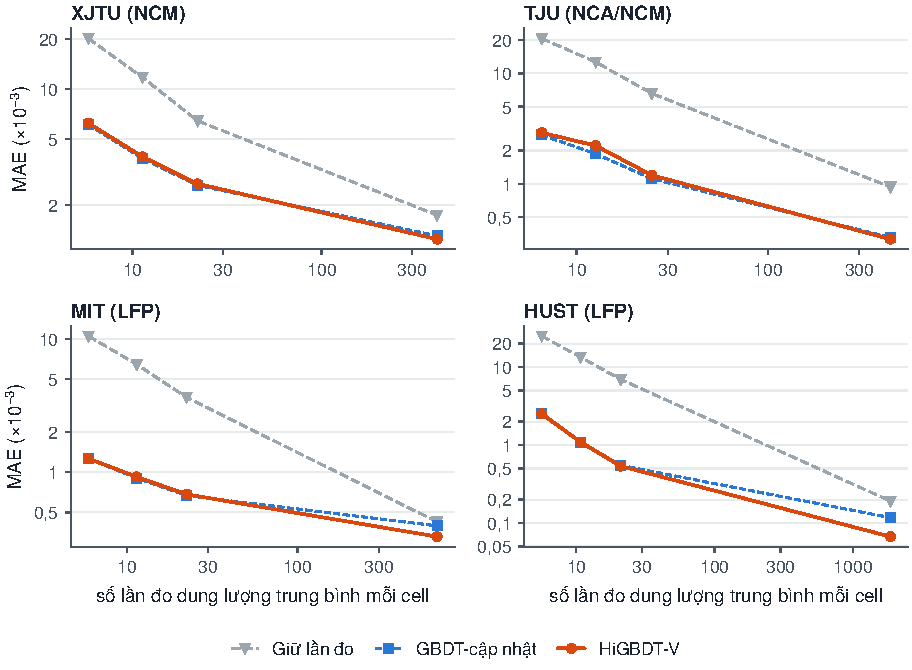
\includegraphics[width=\textwidth]{graphics/fig_e34_cost.pdf}
\caption[Sai số cập nhật theo số lần đo]{MAE ($\times10^{-3}$, thang log) của SOH cập nhật theo số lần đo dung lượng trung bình mỗi cell, bốn lịch đo (mỗi $0{,}2L$, $0{,}1L$, $0{,}05L$ và biết mọi lần đo trước), 30\,\% nhãn, trung bình qua 3 lần lặp. Đường nối chỉ để dễ so, không phải quan hệ liên tục đã ước lượng.}\label{fig:e34cost}
\end{figure}
